\chapter{PortAudio}\label{chap:lib}\label{app:portaudio}
As this project requires the usage of the sound card in a computer some interface is needed. A quick search on Google resulted in a countless number of possibilities for interfacing a C++ program with the sound card of a computer. The team decided on a set of requirements which the interface had to provide. Requirements are listed below:

\begin{itemize}
\item Easy-to-use application programming interface.
\item Detailed documentation
\item Cross platform.
\item Access to raw sample data.
\item Variable sample speed.
\item Support multiple streams.
\end{itemize}

% Introduction .. something about why we need a wrapper to the hardware
The surface of several interfaces was scratched to see what they had to offer. Some of the best possibilities are listed below:

\begin{description}
\item[RT Audio\footnote{}]
\footnotetext{\url{http://www.music.mcgill.ca/~gary/rtaudio/}}
was a good option, as it complies with the requirements and is written in c++, but it has a few disadvantages compared to PortAudio. One of the critical points where RT Audio fails, is the documentation. Though it is present, it is not considered good enough compared to what is presend in the portaudio project. It is also worth bringing to notice, that the API is slightly more complicated then on portaudio.
%The interface is a bit more complicated then on portaudio, and though documentation is present, it is not quite as good as the documentation for portaudio.

\item[QT Multimedia\footnote{}] is developed by Nokia, and is a good suggestion as it comply with the requirements. The disadvantage is that core files from QT itself is needed which result in increased size of the developed software. Not that the size is specified as a requirement of the project itself but it also result in a superior complexity of the developed software itself, so QT Multimedia was discarded.
\footnotetext{\url{http://doc.qt.nokia.com/latest/qtmultimedia.html}}

\item[SDL (Simple Directmedia Layer)\footnote{}]
\footnotetext{\url{http://www.libsdl.org/}}
 is a c library written to provide low-level access to multimedia hardware accross platforms, including audio, video, timers and events. It has wrappers to lot of different languages. It has been developed with the main purpose of use in games and demos.


\item[PortAudio\footnote{}] was finally chosen as the lowermost component of the software as it comply with the requirements mentioned above.  The reason for this final decision was based on the simplicity of the usage of PortAudio. Beside this point it is extremely adaptable which make it possible to use in a wide range of applications. A block diagram can be seen in figure \ref{fig:app_portaudio}.

\footnotetext{\url{http://www.portaudio.com/}}

The research showed a series of suitable libraries to use for this project, but the choise landed on Port Audio as the best solution for the project.

\begin{figure}[!h]
	\begin{center}
	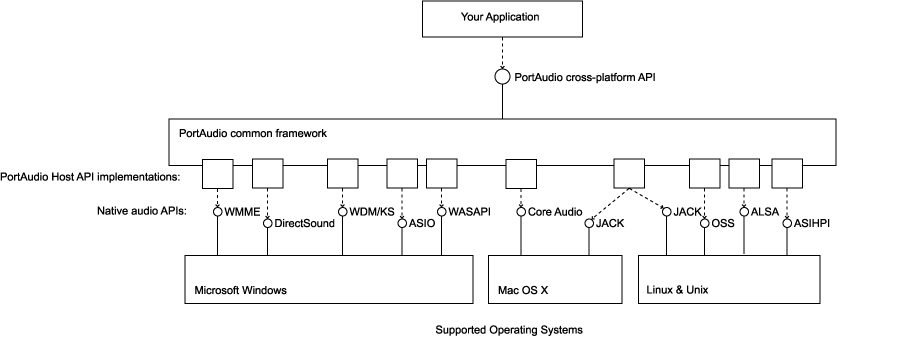
\includegraphics[scale=0.4,trim=0 0 0 0]{content/graphics/appendix/portaudio_architecture.png}%trim=l b r t
	\caption{This is an overview of the PortAudio interface.}
	\label{fig:app_portaudio}
	\end{center}
\end{figure}
\end{description}